\section{Què és?}

Anomenem software privatiu a tot aquell programa publicat sota llicències
que reserven un o tots els drets d'ús, còpia, modificació i distribució
al fabricant qui, pagant, concedeix un ús del programa executable al titular
de la llicència.

Per tant, el software \emph{privatiu} o \emph{propietari} obstrueix la llibertat
de l'usuari final, que quan ha adquirit el programa, té uns drets limitats i fortes
obligacions, que solen incloure la impossibilitat d'adquirir i modificar el codi font del producte
que ell mateix ha comprat, tant com la prohibició total o parcial de la redistribució del programa.
\cite{gnucategories}

\section{Qui el fa?}

El principal desenvolupador de software privatiu a nivell mundial és Microsoft, encara que hi
ha moltes més empreses que també en creen i distribueixen, com \emph{Apple, Oracle, Adobe, VMware,
SAP, Symantec...}\cite{privatiuempreses}

\section{Ús actual}

Avui en dia molta part del software utilitzat per la majoria de població, és privatiu.

Aquesta gran extensió del seu ús és degut a l'inversió milionària al màrketing, i a
pactes amb productors de sistemes operatius i proveïdors d'Internet, que acorden la
prèvia instal·lació de software privatiu als ordinadors. La falta d'informació per
part de la major part d'usuaris fa que aquest fet sigui de poca importància.

\section{Estadístiques d'ús}

\begin{figure}[ht!]
\centering
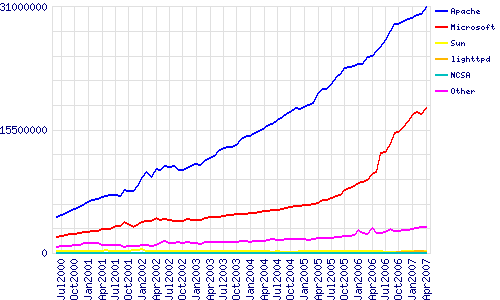
\includegraphics[width=100mm]{data/web_servers_share.png}
\caption{Ús de software privatiu/lliure \cite{whyfoss}}
\label{websshare}
\end{figure}
\begin{figure}[h!]
\centering
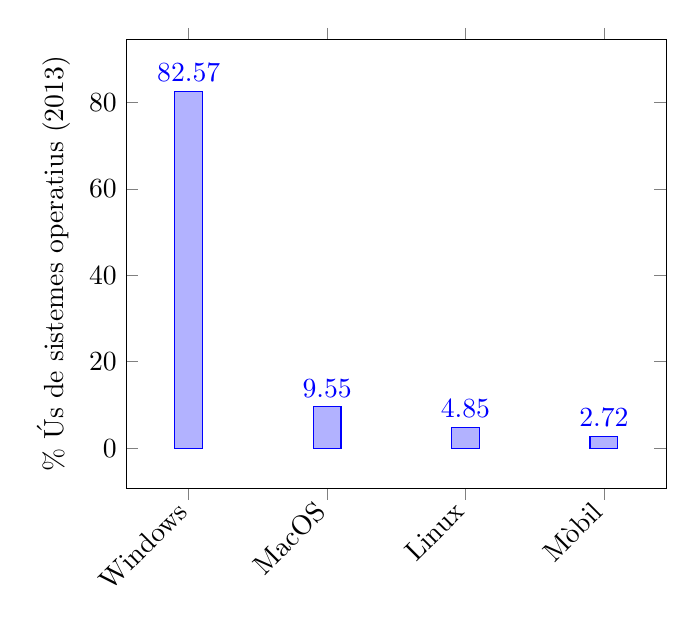
\begin{tikzpicture}
\begin{axis}[
	ybar,
	enlargelimits=0.15,
	legend style={at={(0.5,-0.2)},
	anchor=north,legend columns=-1},
	ylabel={\% Ús de sistemes operatius (2013)},
	symbolic x coords={Windows,MacOS,Linux,Mòbil},
	xtick=data,
	nodes near coords,
	nodes near coords align={vertical},
	x tick label style={rotate=45,anchor=east},
]
\addplot coordinates {(Windows,82.57) (MacOS,9.55)
(Linux,4.85) (Mòbil,2.72)};
\end{axis}
\end{tikzpicture}
\caption{Ús de sistemes operatius \cite{osstats}}
\label{osshare}
\end{figure}

El gràfic \ref{websshare} mostra la distribució (o \emph{market share}) de diferents companyies de software
en l'àmbit dels servidors web. \emph{Apache}\cite{apache} ha mantingut sempre la seva posició,
seguit per \emph{Microsoft} i altres productes. En aquest cas, el software lliure (de la mà de la
llicència \emph{Apache 2.0}\cite{apachelicense}) és prevalent de llarg.

El gràfic \ref{osshare} mostra el market share de \emph{sistemes operatius}


\section{Avantatges de la privacitat}

Ventatges del software privatiu: 

-Propietat i decissió de l'ús del software per part de la empresa: fer un bon software 
requereix una important inversió econòmica que, si fos lliure, no serviria de res ja 
que just quan l'acabéssim, la competència es podria apropiar del mateix.

-Solen tenir millor acabat que el software lliure: en el software lliure, degut a que
 el fa molta gent sol tenir diferències de format i no tenen tan bon acabat (tot i que
 molts softwares lliures tenen molt bon acabat).

-Les aplicacions actuals amb més èxit al mercat són, en majoria, propietaries.

-Més possibilitats en el mercat laboral: en la majoria de les feines d'informàtica la
feina que es durà a terme serà en el softwafare privatiu.
\cite{gentegeek}








